\documentclass[crop,tikz]{standalone}
\usepackage{tikz}

\tikzstyle{baseNode}=[draw,circle,minimum size=15pt,inner sep=0pt]
\tikzstyle{transition}=[-stealth, thick]

\begin{document}
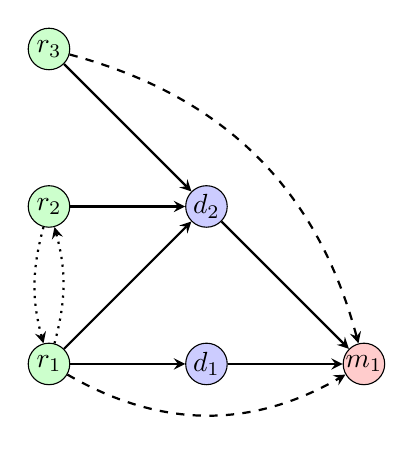
\begin{tikzpicture}

    \node[baseNode,fill=green!20] (r1) at (0, 0) {$r_{1}$};
    \node[baseNode,fill=green!20] (r2) at (0, 2) {$r_{2}$};
    \node[baseNode,fill=green!20] (r3) at (0, 4) {$r_{3}$};
    \node[baseNode,fill=blue!20] (d1) at (2, 0) {$d_{1}$};
    \node[baseNode,fill=blue!20] (d2) at (2, 2) {$d_{2}$};
    \node[baseNode,fill=red!20] (m1) at (4, 0) {$m_{1}$};
    
    
    \draw[transition,dotted] (r1) to[out=75, in=285] (r2);
    \draw[transition,dotted] (r2) to[out=255, in=105] (r1);
    \draw[transition] (r1) to (d1);
    \draw[transition] (r1) to (d2);
    \draw[transition] (r2) to (d2);
    \draw[transition] (r3) to (d2);
    \draw[transition] (d1) to (m1);
    \draw[transition] (d2) to (m1);
    \draw[transition,dashed] (r1) to[out=330, in=210] (m1);
    \draw[transition,dashed] (r3) to[out=345, in=105] (m1);

\end{tikzpicture}
\end{document}